\chapter{Introduction}

% \section{Overview}

\begin{chapquote}{Morpheus, \textit{The Matrix}}
``You take the red pill, you stay in Wonderland, and I show you how deep the rabbit hole goes. Remember, all I'm offering is the truth. Nothing more.''
\end{chapquote}

Reinforcement learning (RL) has shown the capacity to orchestrate or align highly complex generative models, which often proves impossible using supervised learning objectives such as matching distributions or incorporating specific goals into loss functions  \cite{ouyang2022training,lee2023aligning, fan2023dpokreinforcementlearningfinetuning, black2023training, deng2024prdpproximalrewarddifference}. Beyond merely circumventing these challenges, RL should be regarded as a transformative user-model interface endeavor, offering advanced mechanisms for users to explore and manipulate tasks within generative models from a human-computer interaction (HCI) perspective \cite{Du2023-fg, Pommeranz-hci, 10.1145/3357236.3395525}. 
Despite the computational demands and implementation complexities associated with RL, it provides unparalleled flexibility by optimizing arbitrary expected rewards, where the reward can be a non-differentiable scalar function or a model trained using human feedback. This becomes particularly relevant in the context of large models like LLMs \cite{wan2024efficientlargelanguagemodels} and diffusion models \cite{karras2022elucidatingdesignspacediffusionbased, song2021scorebasedgenerativemodelingstochastic, Salimans2022ProgressiveDF, watson2021learningefficientlysamplediffusion, watson2022learningfastsamplersdiffusion}, which have driven significant research towards improving sample efficiency and prioritizing inference. These advancements make the exploration of RL agents atop these generative models especially compelling. \\

\noindent An agent in the context of RL is a decision-making entity that interacts with an environment, learning to take actions that maximize cumulative reward. Conversely, a diffusion model excels at learning highly 
complex distributions, enabling it to generate samples from the learned 
distribution.  This allows us to interpret the diffusion model as an agent that interacts with the environment to generate samples, with the goal of maximizing a desired attribute, such as compressibility or aesthetic quality, as measured by a reward function. Figure~\ref{fig:anatomy-rl-algo} illustrates this process: it begins with generating a set of samples using a pretrained diffusion model, followed by obtaining rewards that measure the alignment of each generation with the task goal. The next step involves fitting a model by estimating the gradients of the expected reward of the samples with respect to the diffusion model parameters. Finally, these estimates are used to update the model parameters, directing the diffusion model to generate samples with higher expected returns. When executed correctly, this iterative process results in a generative model that is aligned with the goal encoded it the reward signal. \\

\noindent In this thesis, we explore the application of reinforcement learning techniques to adapt pretrained diffusion models for new tasks. We provide the necessary background to understand the intersection of diffusion models and policy gradient methods from the field of reinforcement learning, aiming to serve as a comprehensive guide for those looking to contribute to this area. We then implement the iterative process depicted in Figure~\ref{fig:anatomy-rl-algo}, based on the work \textit{``Training Diffusion Models with Reinforcement Learning''} (Black, 2023 \cite{black2023training}), which introduces policy optimization algorithms in the realm of diffusion models (DDPO). \\

\noindent Using the pretrained model \href{https://huggingface.co/google/ddpm-celebahq-256}{\textit{google/ddpm-celebahq-256}} trained with a foundational diffusion model approach (DDPM) \cite{ho2020denoising}, we 
simplify the understanding of the core components in the fine-tuning process. We explore the effect of extending the rewards over the generation process instead of focusing solely on the final sample and incorporate a control variate method. The code, model checkpoints, and training dynamics are provided with this work (see Appendix~\ref{appendix:implementation}). 

\begin{figure}[ht]
  \centering
  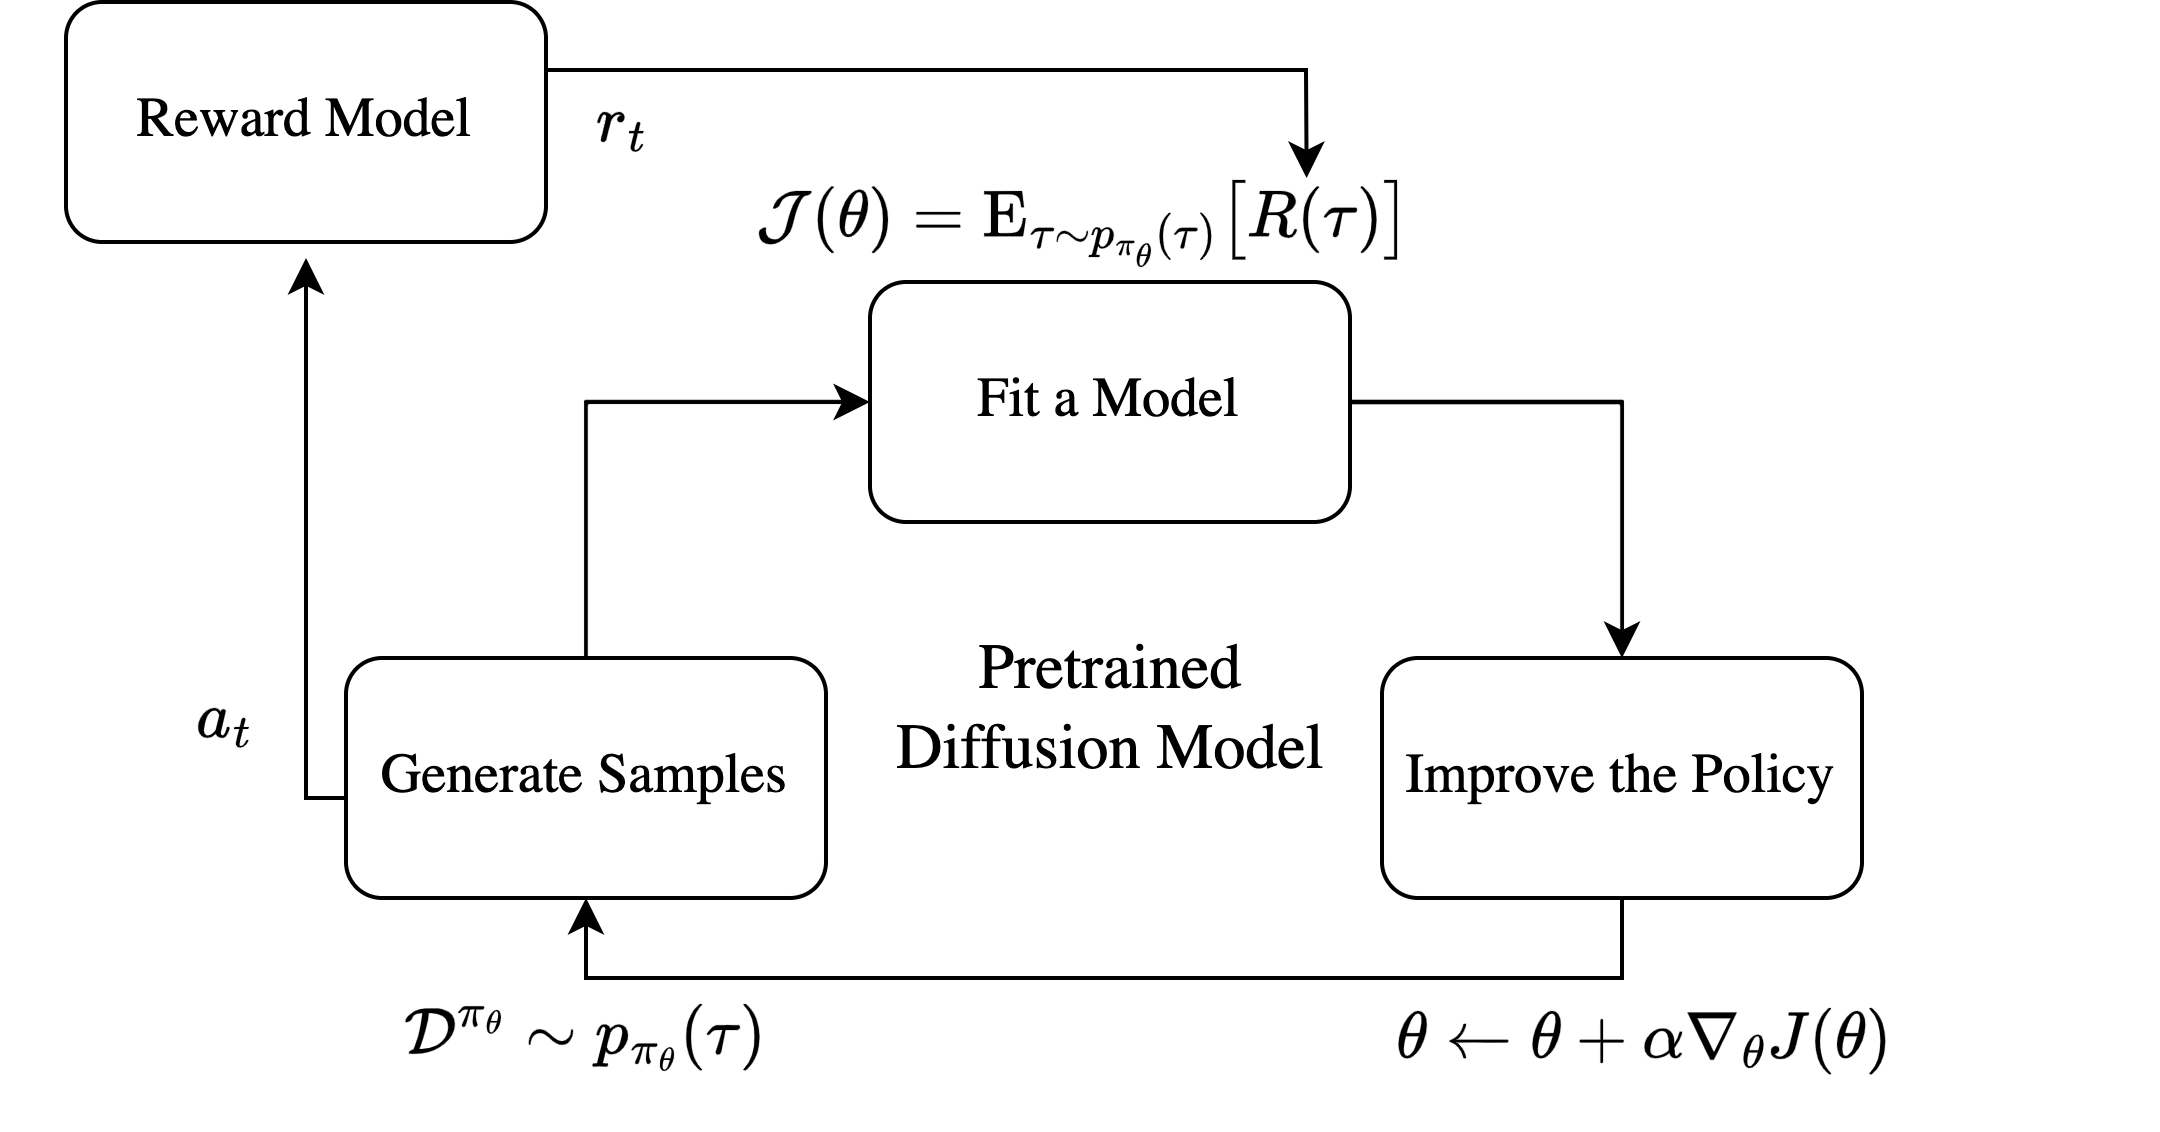
\includegraphics[scale=0.85]{ch3-rl/anatomy-rlhf-algorithms.png}
  \captionsetup{width=\textwidth} % set the width of the caption
  \caption{\textbf{Iterative process of finetuning a diffusion model using reinforcement learning}. The process consists of three stages: (i) collecting a dataset of generated samples $\mathcal{D}^{\pi_{\theta}}$ using the dffusion model, (ii) estimating the gradient of the expected return from the dataset using Monte Carlo estimation, and (iii) optimizing the diffusion model using the estimated gradient. A reward model based on human feedback can be employed to estimate the reward of the actions. In this case, the diffusion model is finetuned using reinforcement learning from human feedback (RLHF).}
  \label{fig:anatomy-rl-algo}
\end{figure}


\section{Related Work}

\noindent\textbf{Diffusion Models.} Diffusion models and score-based models represent a significant advancement in the field of generative models. These models learn a distribution $p(\mathrm{x})$ from a dataset $\mathcal{D}$, enabling evaluation and sampling of complex data types such as images or audio. They begin with a simple prior distribution (e.g., isotropic-Gaussian) and iteratively transform it into the target distribution through a denoising process. Recent advancements have focused on making the sampling process more efficient \cite{song2020denoising, nichol2021improved, Salimans2022ProgressiveDF}. The progress in diffusion models has led to impressive results in tasks like text-conditional image generation \cite{ramesh2022hierarchical, saharia2022photorealistic}, super-resolution, in-painting, style transfer, and combining different data modalities. \\

\noindent\textbf{Controling Diffusion Models.} Controlling diffusion models for new tasks is a challenging and evolving area of research. Given the high cost and resources required to train generative models from scratch, adapting pretrained diffusion models is crucial. This adaptation allows the models to learn new concepts, such as specific objects or scenes, with minimal data. Techniques like using a small set of images to teach a model new concepts without losing its diversity \cite{ruiz2023dreambooth}, and textual inversion to embed new concepts \cite{gal2022image}, have shown promising results. Additionally, ControlNet provides advanced control over the generation process, enabling inputs like canny edges \cite{zhang2023adding}. However, many downstream tasks cannot be easily expressed through text prompts or loss functions due to their context-dependent or subjective nature. \\
% \ca{Condition a model during training based on text to give flexibility, condition during inference with classifier guidance, using an external classifier to guide the generation process...} \\

% \noindent\textbf{Reinforcement Learning \& Diffusion Models.} Citar trabajos de Schulman \citep{schulman2015trust} y \citep{schulman2017proximal}. The former work extend a theoretical lower bound that works for policy update, original present for the case of mixture policies (something between $\pi_{old}$ and $\pi`$), and now adapted to stochastic policies. They introduce a distance measure between policies: total variation divergence. In the following section, we will detailed more the policy optimization approach for finetuned diffusion models with RL. \ca{}\\

\noindent\textbf{Reinforcement Learning from Human Feedback (RLHF).} Recently the attention to use human feedback in reinforcement learning has increased \cite{kaufmann2023survey}. The core idea is to capture the human feedback into a reward model that can be used to train the policy that dictates the agent's behaviour. The benefits it's to allow different types of feedback, such as binary, continuous, or even more complex signals that can be used to train in a supervised learning fashion. Then, instead of design the reward function---\textit{or use feature engineering}---we can gives the agent access to the reward model to obtain the neccessary feedback for trajectories and optimize its behaviour to learn the task. \\


%\noindent Diffusion \citep{sohldickstein2015deep} \citep{ho2020denoising} and score-based models \citep{song2020generative} are a kind of generative models, in which they learn from the dataset $\mathcal{D}$ a distribution $p(\mathbf{x})$ and achieve the two basic primitive operations expected for this type of models, evaluation and sampling, with the importance that scale well and handle highly complex data such as images or audio. To accomplish this task, diffusion models start with a simple prior distribution (e.g. isotropic-gaussian) and, iteratively, through a denoising process, it mutates into the target distribution. Recent years have shown an essential advance in extending and adapting the work on diffusion models, likewise making the sampling process faster in the work of \cite{song2020denoising}, \cite{nichol2021improved}, and \cite{Salimans2022ProgressiveDF}. Incorporate additional information $\mathbf{y}$ (e.g. text prompt, an image seed) to learn a conditional model $p(\mathbf{x} | \mathbf{y})$; this endeavour will be explored indirectly by guiding the sampling with an external classifier in \cite{Dhariwal2021DiffusionMB}, or achieving the same but directly in the model training phase using classifier-free guidance purpose in \cite{Ho2022ClassifierFreeDG} and effectively implemented in work \cite{nichol2022glide}. These techniques had many connections with the concept of temperature commonly used in Large Language Models (LLM) and proved helpful to guide the sampling in the gradient direction toward the space between $\mathbf{x}$ and $\mathbf{y}$ signals. Moreover, progress toward improving the likelihood estimation and exhibited impressive results on tasks such as text conditional image generation with visual language models \cite{ramesh2022hierarchical} and \cite{saharia2022photorealistic}, super-resolution \cite{ho2021cascaded}, in-painting, style transfer, and combining different data modalities. \\

%\noindent A vital research line is to use pre-trained diffusion models and adapt to novel tasks or concepts. Given the high cost of data recollection, the quantity and quality of these, and the computational resources it takes to train these "lossless" generative models from scratch. The idea is to push forward in the line that follows the LLM and their adaptation to downstream tasks \citep{Radford2019LanguageMA}. Specifically, the work of \cite{ruiz2023dreambooth} using a small number of images 3-5 of a new concept, such as a specific person, pet, or landscape, shows that a pre-trained model can learn it without sacrificing the current diversity of the model and edit the new concept or inserted it into another context (e.g. my pet surfing in Hawaii). Same goal but a different approach, \cite{gal2022image} proposed textual inversion to learn a textual embedding of the new concept, and \cite{zhang2023adding} go further with ControlNet, which not only allows you to learn a new concept with a pre-trained model but gives you additional input controls for the generation process such as canny edges. Research such as \cite{shi2023instantbooth} use adapter layers in the model architecture to reinforce the signal of the new concept without compromising the model's capabilities, in which a block is appended into the model architecture with the necessary set of weights to re-interpreted the model inference toward a signal, or more generally, a new task. However, only some downstream tasks can be easily expressed using a text prompt or a loss function. Other tasks are heavily context-dependent, challenging to define, or directly subjective. Recent work by \cite{black2023training} brings Reinforcement Learning techniques for adapting pre-trained diffusion models with challenging objectives to control via prompting, such as image compressibility or prompt alignment, and achieve promising results. Borrowing ideas from previous work and the recent development in Reinforcement Learning Human Feedback (RLHF) used by visual language models \citep{lee2023aligning}, this thesis work aims to continue this research line to fine-tuning diffusion models via rewards functions. \\

\section{Contributions and Outline}


This thesis explores the application of Reinforcement Learning (RL) techniques to adapt pretrained diffusion models for new tasks. Specifically, it involves optimizing policies for agents built on top of the denoising network within the diffusion model framework. This approach guides the sampling process to maximize a reward signal. The main contributions of this work are: \\


\begin{enumerate}
    \item Offering the necessary background to understand the intersection of diffusion models and reinforcement learning, serving as a comprehensive guide for those looking to contribute to the field.
    \item Reproducing the study \textit{``Training Diffusion Models with Reinforcement Learning''} (Black, 2023 \cite{black2023training}), which introduces policy optimization algorithms (DDPO) for adapting pretrained diffusion models to new tasks.
    \item Empirical Analysis of Reward Signals: Conducting empirical analyses of reward signals during the sample trajectories within the diffusion process.
    % \item Presenting I-DDPO, an extended approach that considers rewards of intermediate states in the diffusion process and includes a value function to approximate a baseline.
    \item Human Feedback Integration: Demonstrating how human feedback can be incorporated into the loop via the reward model to provide guidance and align model objectives.
\end{enumerate}

\noindent To lay the groundwork, \textbf{Chapter 2} covers the basics of diffusion models, including their formulation as a Markov chain, the training objective, conditioning information or guiding model sample generation, and improvements such as speeding up sample generation. \\

\noindent Next, a broad overview of the Reinforcement Learning field is provided in \textbf{Chapter 3}, focusing on Markov Decision Processes (MDP) and Policy Optimization algorithms. The goal is to understand how to train an agent to take actions in response to its environment. \\

\noindent Equipped with the necessary background, the intersection of diffusion models and reinforcement learning is explored in \textbf{Chapter 4}. This includes reproducing the Denoising Diffusion Policy Optimization (DDPO) \cite{black2023training} using a smaller unconditional generative model and discussing the challenges and opportunities of this approach. 

%Then, we will introduce I-DDPO that consider rewards of the intermediate state in the diffusion process and includes a value function to approximate a baseline. Improving the Monte Carlo estimate of the gradient. %\ca{Afinar el párrafo del capítulo } \\

\noindent Finally, \textbf{Chapter 5} presents the conclusions of this work. 